\begin{flushleft}

The string interpreter is one of the major components of the L-system, the L-system rewriter takes an L-system input and carries out a set of production rules and eventually provides the resulting string of modules. The rewriter forms the overall structure and calculates the values of any module parameters that will be used within the string interpreter, however, up until this point the string of modules does not hold any particular meaning, it is simply the result of a set of production rules. The string interpreter interprets the string of modules and in a way that is serves its purpose within the problem domain. This chapter will outline a string interpreter for generating 3D models of plant structures as well as simulating gravity and wind in real time on the plant models. 

\vspace{5mm}



\end{flushleft}

\section{Turtle Interpretation}

\begin{flushleft}



\end{flushleft}

\section{Displaying the L-system Instructions} \label{Display L-system Instructions}

\subsection{Basic 2D L-systems} 

There are a number of fractal geometry that have become well known particularly with regards to how they can seemingly imitate nature \cite{mandelbrot1982fractal}. Particularly with the geometry such as the Koch snowflake which can be represented using the following L-system.

\begin{figure}[htbp]
	\raggedright
	\textbf{\underline{Koch Curve:}} \\
	\#n = 4; \\
	\#define r 90; \\
	\#w : F(1); \\
	\#p1 : F(x) : * : F(x)+(r)F(x)-(r)F(x)-(r)F(x)+(r)F(x);\\
	{\centering
		\vspace{7px}
		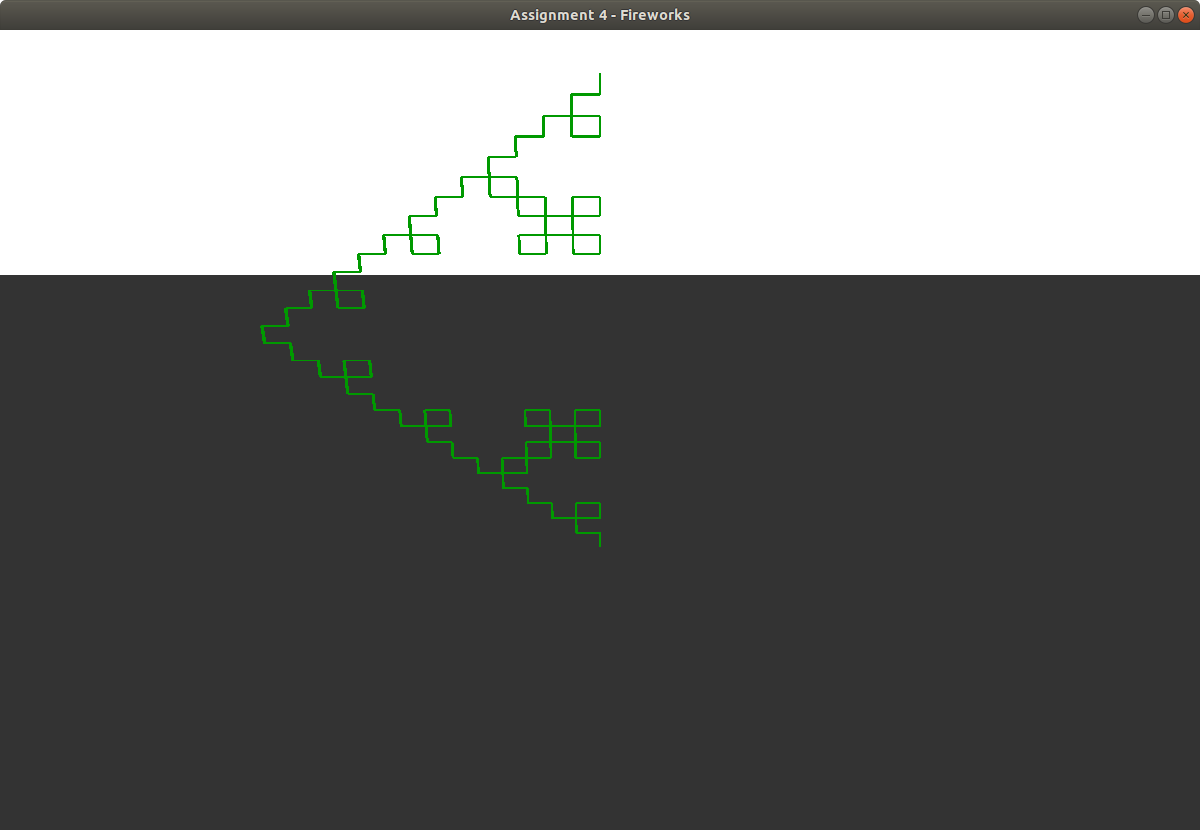
\includegraphics[scale=0.15]{KochCurve/KochCurve04.png}
		\caption{Koch Curve.}
	}
\end{figure}
\begin{figure}[htbp]
	\raggedright
	\textbf{\underline{Sierpinski Triangle:}} \\
	\#n = 4;\\
	\#define r 60;\\
	\#w : F(1);\\
	\#p1 : F(x) : * : X(x)-(r)F(x)-(r)X(x);\\
	\#p2 : X(x) : * : F(x)+(r)X(x)+(r)F(x);\\
	{\centering
		\vspace{7px}
		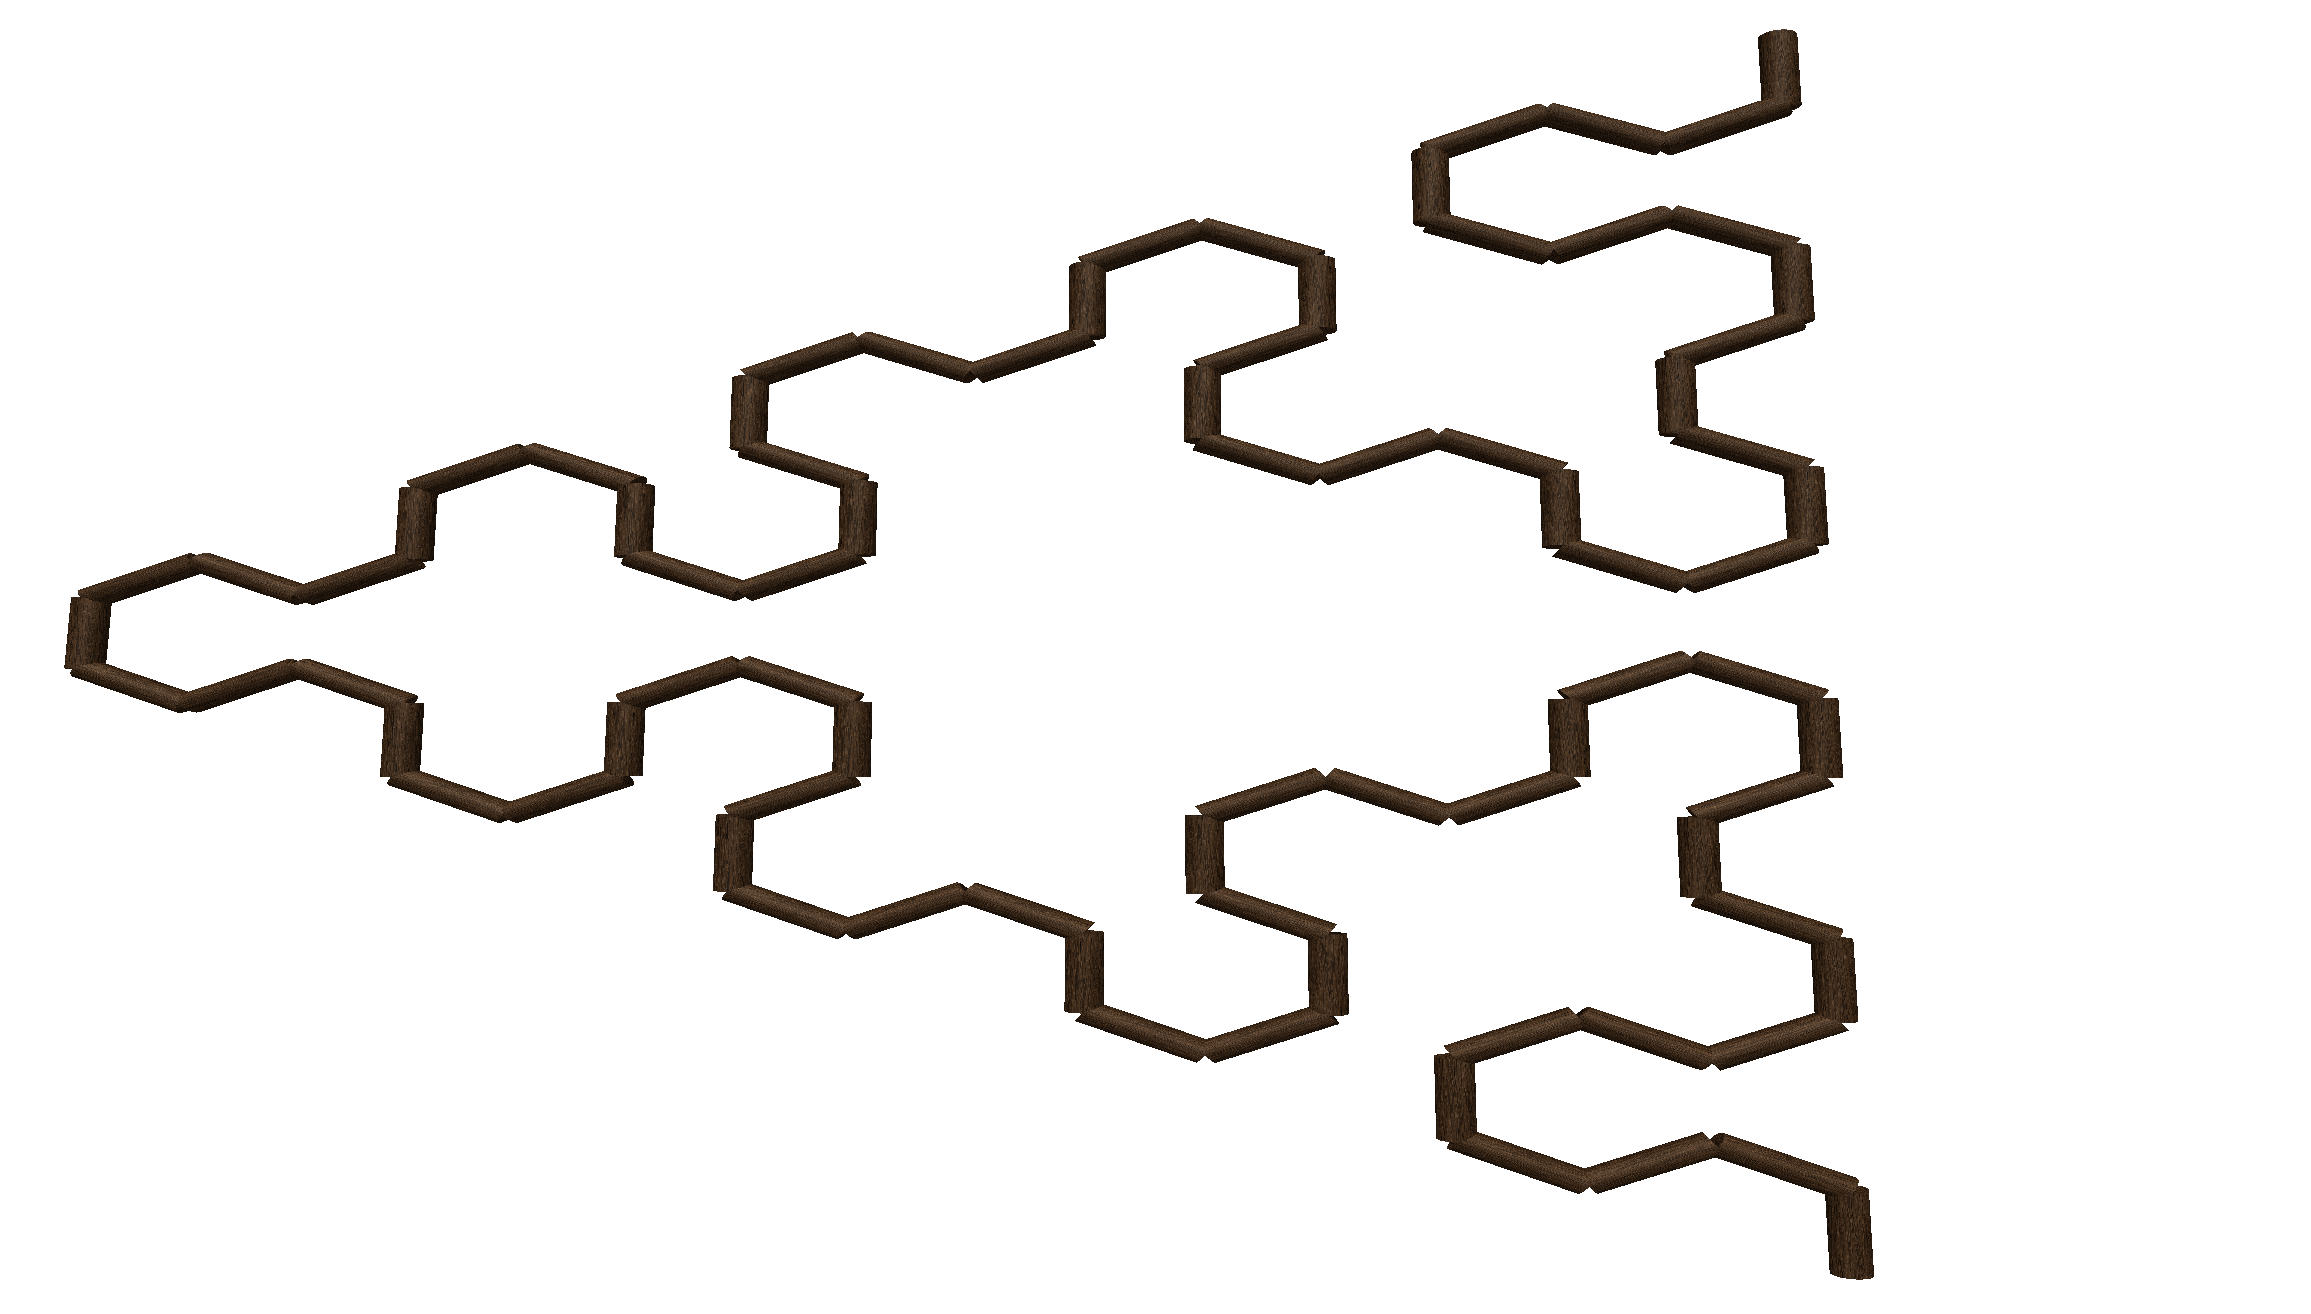
\includegraphics[scale=0.15]{SierpinskiTriangle/SierpinskiTriangle04.png}
		\caption{Sierpinski Triangle.}
	}
\end{figure}
\begin{figure}[htbp]
	\raggedright
	\textbf{\underline{Fractal Plant:}} \\
	\textbf{Alphabet:} X, F\\
	\textbf{Constants:} +, -, [, ] \\
	\textbf{Axiom:} X \\
	\textbf{Angle:} 25$^\circ$ \\
	\textbf{Rules:} \\
	X $\rightarrow$ F-[[X]+X]+F[+FX]-X\\
	F $\rightarrow$ FF \\
	{\centering
		\vspace{7px}
		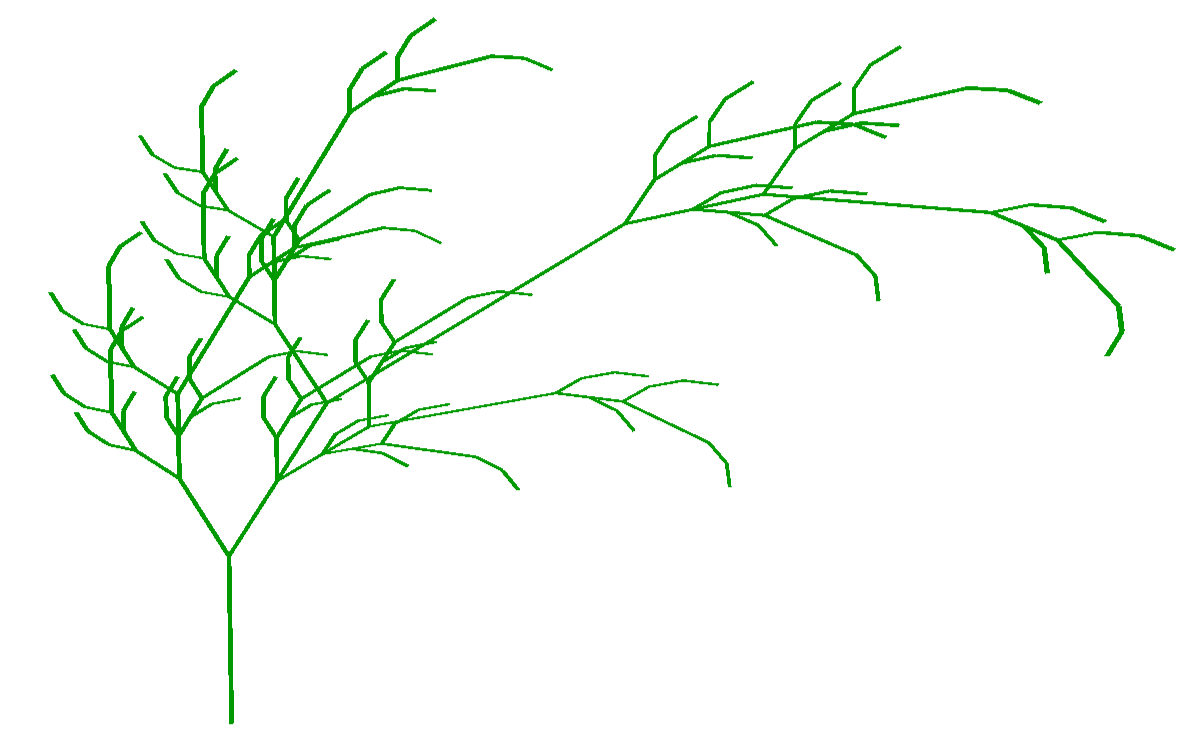
\includegraphics[scale=0.15]{FractalPlant/FractalPlant05.png}
		\caption{Fractal Plant.}
	}
\end{figure}
\begin{figure}[htbp]
	\raggedright
	\textbf{\underline{Fractal Bush:}} \\
	\textbf{Alphabet:} F\\
	\textbf{Constants:} +, -, [, ] \\
	\textbf{Axiom:} F \\
	\textbf{Angle:} 25$^\circ$ \\
	\textbf{Rules:} \\
	F $\rightarrow$ FF+[+F-F-F]-[-F+F+F]\\
	{\centering
		\vspace{7px}
		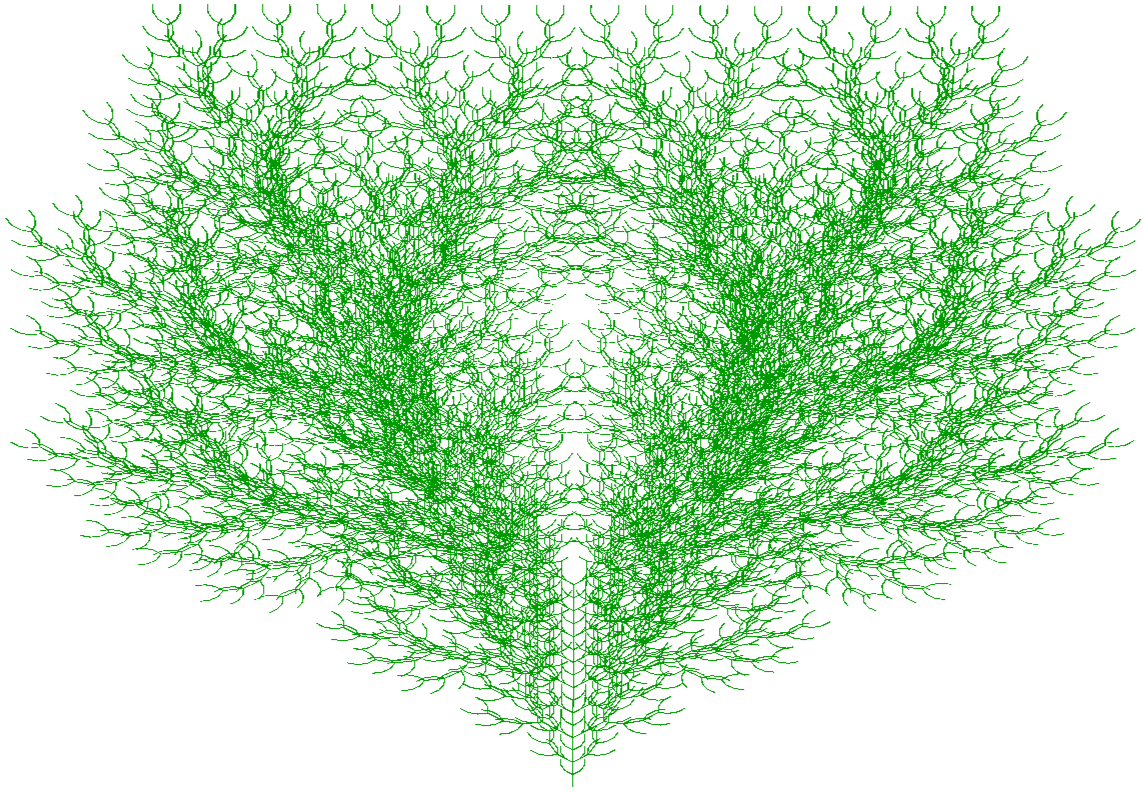
\includegraphics[scale=0.15]{FractalBush/FractalBush06.png}
		\caption{Fractal Bush.}
	}
\end{figure}

\FloatBarrier

\subsection{The Use of L-systems in 3D applications}

\begin{flushleft}

L-systems have been talked about and researched since its inception in 1968 by Aristid Lindenmayer. Over the years it's usefulness in modelling different types of plant life has been very clear, however its presence has been quite absent from any mainstream game engines for the most part, these engines relying either on digital artists skill to develop individual plants or on 3rd party software such as SpeedTree. These types of software use a multitude of different techniques however their methods are heavily rooted in Lindenmayer Systems. 

\end{flushleft}


\section{Modeling Seamless Branches}

\begin{flushleft}

Modeling the branches of a plant is the most important part behind the overall look and feel of that plant. The L-system described in the previous sections is able to describe the most important details about the plants structure. For instance the width, length, weight and other important information. Our job now is to take this information and intelligently generate a model consisting of vertices, normals, texture coordinates and other information that can then be provided to the GPU and then rendered on the screen.\\

\vspace{5mm}

The most obvious way to generate a model for a branching structure would be to take a number of cylinders and to rotate and stack them according to the branching structure. In this way we are able to represent the overall branching structure of the tree. However there is a problem pointed out by Baele and Warz\'{e}e "The branches junction causes a continuity problem: to simply stack up cylinders generates a gap" \cite{baele2005real}. This can be shown in the figure below:

\FloatBarrier

\begin{figure}[htbp]
	{\centering
		\vspace{7px}
		\setlength{\fboxrule}{1pt}
		\fbox{
			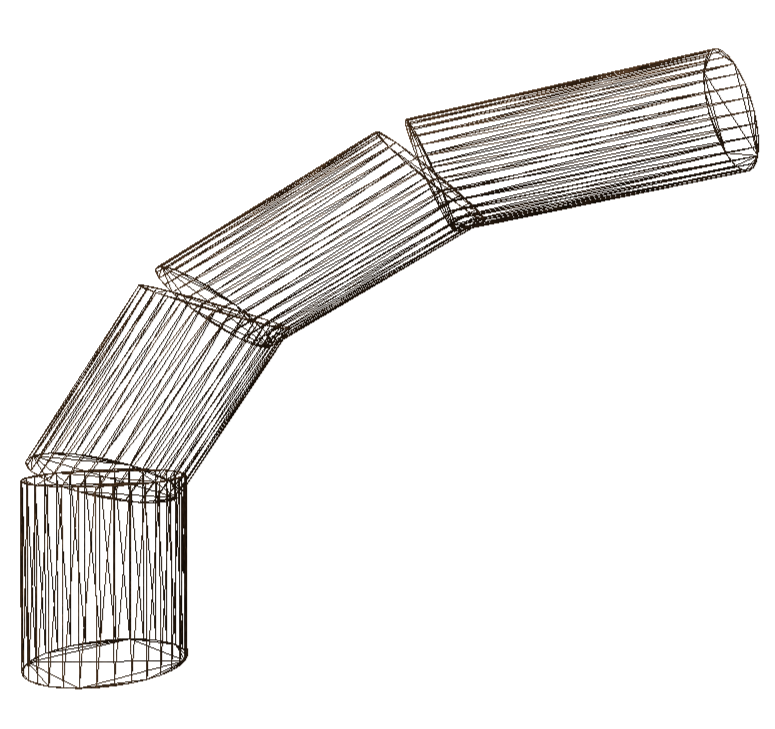
\includegraphics[scale=0.16]{Diagrams/stackedBranchesMesh.png}
		}
		\caption{Example of the continuity problem faced with stacked branching with a 25$^{\circ}$ bend per joint.}
	}
\end{figure}

\FloatBarrier

\vspace{5mm}


\vspace{5mm}

This simple method of stacking cylinders gives a reasonable looking tree structure and it is usually good enough when the angles of branches are not more than about 25$^{\circ}$ and the size of the branches do not change. However for a much more convincing tree structure we will want to do better than this. The logical next step would be to actively link the branch segments together.

\FloatBarrier

\begin{figure}[htbp]
	{\centering
		\vspace{7px}
		\setlength{\fboxrule}{1pt}
		\fbox{
			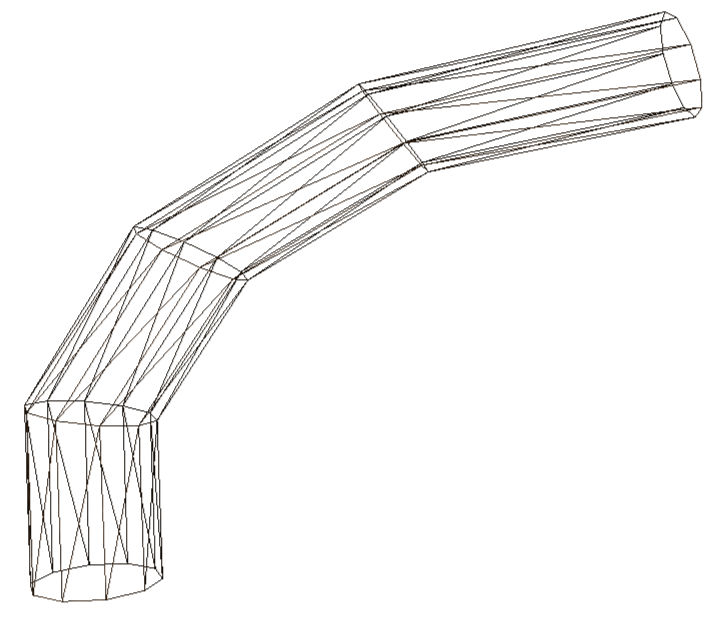
\includegraphics[scale=0.16]{Diagrams/linkedBranchesMesh.png}
		}
		\caption{Example of linked branching with a 25$^{\circ}$ bend per joint.}
	}
\end{figure}

\FloatBarrier

\end{flushleft}